\chapter{Systementwurf}\label{chp:systementwurf}


%#######################################################################################
%#######################################################################################
\section{Variantenmanagement und Parameter}
\paragraph{}

Die Lösung zum Speichern und Darstellen der Parameterwerte abhängig von der aktiven Variante wird im diesem Kapitel erläutert.\\

\begin{figure}[h!]
  \begin{center}
    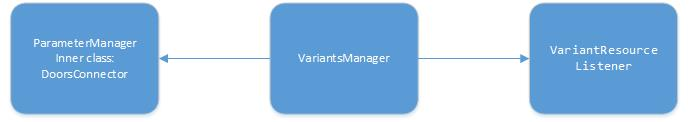
\includegraphics[scale=0.7]{5_1_klassenuebersicht.jpg}
  		  \caption{Einfache Übersicht der Klassen}
     \label{ttn.verbindung.klassen.loesung}
  \end{center}
\end{figure}


Die genaue Darstellung der Klassen befindet sich im Anhang  \ref{A.PM.Diagramm}. Ablauf für das Speichern eines Parameters in einem Baumelement:
\begin{enumerate}
\item Der Benutzer verknüpft eine Anforderung an ein Baumelement.
\item Der \textit{Listener} meldet, dass eine Änderung vorgenommen wird und gibt die Informationen weiter.
\item Der \textit{VariantsManager} lädt und übergibt die nötigen Informationen an den \textit{ParameterManager}.
\item Der \textit{ParameterManager} lädt, sucht und erstellt ein \textit{ParameterTag}  und gibt den Befehl, dass ein \textit{ParameterTag} an ein Baumelement hinzugefügt werden muss.
\item Der \textit{ParameterManager} gibt den Befehl an den \textit{Listener} weiter.
\item Der Befehl wird an die Befehlskette angehängt.
\end{enumerate}

In den nächsten Unterkapiteln wird die Aufgaben der jeweiligen Klassen erläutert und der Ablauf ausführlicher erklärt.


%#######################################################################################
\subsection{VariantsManager}\label{sub.VariantsManager}
Die Hauptaufgabe des \textit{VariantsManager} ist die Zuordnung der Varianten. Hier werden Baumelemente zu Varianten hinzugefügt und gelöscht. Dabei muss der Klassifikationsbaum neu gezeichnet werden. Diese Klasse kümmert sich auch um die Umschaltung zwischen Varianten in der Variantenansicht (siehe Abbildung \ref{ttn.generic}) und um die richtige Darstellung der Baumelemente mit aktuellen Informationen.\\


Für die  Zwecke dieser Arbeit wurde die Klasse erweitert. Um die Aufgaben dieser Klasse zu erläutern, wird der Vorgang des Hinzufügen eines Parameters an einem Baumelement dargestellt. Der \textit{VariantsManager} setzt die Baumelement - ID und die Anforderungskennung in der Klasse \textit{ParameterManager}. Die Klasse dient als Schnittstelle zwischen dem \textit{Listener} (siehe Kapitel \ref{sub:RSListner}) und der Klasse \textit{ParameterManager}  (siehe Kapitel \ref{sub:ParameterManager}).\\


Der \textit{Listener} hat die Aufgabe dem \textit{VariantsManager} zu melden, wenn eine Änderung\footnote{Aktionen werden vom Benutzer ausgelöst anhand von Bedienelemente in der Benutzeroberfläche.} geschehen wird oder geschehen ist. Im \textit{Listener} werden die benötigten Informationen gefiltert und an die Klasse weitergegeben, damit Änderung vorgenommen werden können. Im Fall der Parameterersetzung sind  die Identifikationsnummer eines Baumelementes und die Anforderungskennung der verlinkten Anforderung. Diese beiden Kennungen dienen dazu, dass der \textit{VariantsManager} die jeweiligen Objekte (ein Baumelement und eine Anforderung) laden kann. Diese Objekte werden dann der Klasse \textit{ParameterManager} übergeben.\\


Das angesprochene Baumelement muss aus dem TESTONA-Diagramm geladen werden. Anhand der Identifikationsnummer werden die verschiedenen Baumelemente einzeln abgefragt bis das richtige Baumelement gefunden wurde. Danach wird das Baumelement dem ParameterManager Objekt übergeben.\\


Im Fall von der Anforderungskennung, werden mehrere Informationen übergeben. Die Anforderungskennung wird in einer lokalen Variablen vom \textit{ParameterManager} Objekt gespeichert. Damit der Inhalt der Anforderung gelesen werden kann, müssen alle in TESTONA gespeicherte Anforderung dem \textit{ParameterManager} Objekt übergeben werden. Die gespeicherten \textit{Tags} des TESTONA"=Objekts werden abfragt, um folgende Objekte an das \textit{ParameterManager} Objekt übergeben zu können:


\begin{itemize}
\item \textbf{RequirementsConnetionTag}: beinhaltet die Information zur Datenbankverbindung, unter anderem die Verbindungsidentifikation (DOORS), das Modul(Tabelle) in der die Anforderung gespeichert ist und die Schnittstelle zur Datenbank. Anhand dieser Informationen wird später die Verbindung zur Datenbank aufgebaut.

\item \textbf{RequirementsListTag}: ist eine \textit{Map} mit allen in TESTONA gespeicherten Anforderungen. Das \textit{Key} ist die Anforderungsidentifikationsnummer und der Wert der Inhalt der Anforderung. Eine Anforderung aus dieser Liste wurde mit dem Baumelement verknüpft.

\item \textbf{VariantListTag}: ist eine Liste mit allen in TESTONA definierten Varianten.
\end{itemize}


Anhand dieser Informationen kann die Klasse \textit{ParameterManager} ein Parameter an ein Baumelement hinzufügen. Parameter können nicht nur hinzugefügt werden, sondern auch gelöscht werden. Ein Parameter wird aus einem Baumelement gelöscht, indem die verknüpfte Anforderung vom Baumelement entfernt wird. Der Ablauf für das Löschen eines Parameter ist im Grunde der gleiche wie beim Hinzufügen. Als nächstes werden die Funktionen des \textit{Listeners} erörtert.




%#######################################################################################
\subsection{ResourceSetListener}\label{sub:RSListner}
Wenn der Benutzer eine Anforderung mit einem Baumelement verknüpft, dann muss der \textit{Listener} das Geschehen abfangen. Er muss so programmiert werden, dass das Interface \textit{ResourceSetListener}\footnote{http://download.eclipse.org/modeling/emf/transaction/javadoc/1.0.3/org/eclipse/emf/transaction/ ResourceSetListener.html} implementiert wird. Da der \textit{VariantsManager} einen solchen \textit{Listener} bereits besitzt, wurde dieser lediglich erweitert. Die Aufgabe des \textit{ResourceSetListener} ist, den Benutzer zu benachrichtigen, wenn sich eine Ressource ändert. Der \textit{Listener}  \glqq horcht\grqq~ auf die ankommenden Nachrichten (\textit{ResourceSetChangeEvent}) und wertet den Inhalt dieses Events aus.\\

Der \textit{Listener} implementiert zwei Methoden, die für das Abfragen der Events relevant sind. Eine davon heißt \textit{resourceSetChanged(Event e)}. Diese Methode wird aufgerufen, wenn sich eine Ressource ändert. Am Anfang wurde diese Methode  für das Abhören von Events (wenn eine Anforderung zu einem Baumelement verknüpft wird) favorisiert, um danach die Parameterersetzung zu triggern. Nach der Implementierung konnte ich feststellen, dass die Methode keine Schreibrechte auf die Baumelemente besitzt. Da sich die Ressource zu diesem Zeitpunkt schon geändert hatte.\\


Um die Schreibrechte zu besitzen, habe ich dann die Methode \textit{transactionAboutToCommit(Event e)} betrachtet. Diese Methode wird aufgerufen, bevor eine Änderung vorgenommen wurde. Es erfolgt eine Benachrichtigung, dass eine Änderung erfolgt ist und welche Objekte (ein Baumelement und die angehängte Anforderung) betrachtet werden. Zu diesem Zeitpunkt besitzt die Klasse noch Schreibrechte auf die Baumelemente und kann die Änderung vornehmen. Außerdem hat diese Methode als Rückgabewert ein \textit{Command}. So können Kommandos an der Commandstack angekettet werden. Dank der Anordnung des Commadstacks wird der Befehl, ein Parameter an ein Baumelement hinzuzufügen, zum richtigen Zeitpunkt ausgeführt. Mehr Informationen zu Kommandos werden in Kapitel \ref{sub.Command} aufgeführt.


Die empfangene Nachricht beinhaltet folgende Elemente: 

\begin{itemize}
\item \textbf{Event: }ResourceSetChangeEvent, die Ressourcen des Objektes haben sich geändert,
\item \textbf{Notifier: } welches Objekt schickt die Nachricht,
\item \textbf{Notification: }Beschreibung der Änderung im \textit{Notifier},
\item \textbf{OldValue: } alter Wert, wenn nicht vorhanden \textit{null},
\item \textbf{NewValue: } neuer Wert, beim Löschen von Werten \textit{null}.
\end{itemize}


Jetzt wird als erstes der \textit{Notifier} abgefragt, um auswerten zu können, ob die Nachricht relevant ist. Es müssen drei Fälle unterschieden werden. Eine Anforderung wird:


\begin{enumerate}
\item zum ersten Mal an einem Baumelement verknüpft,
\item an einem Baumelement verknüpft, an dem schon andere Anforderungen verknüpft sind,
\item gelöscht.
\end{enumerate}


In allen drei Fällen muss der \textit{Listener} wissen, an welchem Element  das Event ausgelöst wurde und welche Anforderung hinzugefügt oder gelöscht wurde. Zu diesem Zeitpunkt kann noch nicht festgestellt werden, ob in der Anforderung bereits ein Parameter definiert ist.\\


\subsubsection{Eine Anforderung hinzufügen}
Ist der \textit{Notifier} eine Instanz von \textit{TestonaClass}, so wurde eine Anforderung zum ersten Mal an ein Baumelement verknüpft oder gelöscht. Um unterscheiden zu können, werden die Werte von \textit{NewValue} und \textit{OldValue} ausgewertet. Wenn \textit{NewValue} eine Instanz von \textit{RequirementTag} ist, dann wurde eine Anforderung hinzugefügt. Aus dem \textit{Notifier} wird die ID (repräsentiert das Baumelement) und aus der Variable \textit{NewValue} die Anforderungskennung (diese wurde in DOORS vergeben) abgefragt. Beide Werte werden dem \textit{VariantsManager} weitergegeben, um danach den Befehl als Rückgabewert für das Hinzufügen eines \textit{ParameterTags} zu bekommen.\\


Der Befehl wird nicht sofort als Rückgabewert der Methode \textit{transactionAboutToCommit} weitergegeben. Der Grund für diese Maßnahme heißt, dass der Rückgabewert auch \textit{null} sein kann. Wenn kein Parameter in der Anforderung definiert ist, so muss auch kein \textit{ParameterTag} an das Baumelement hinzugefügt werden und es muss kein Kommando ausgeführt werden. In der Methode \textit{transactionAboutToCommit} werden auch andere \textit{Events} ausgewertet, die ebenfalls Kommandos ausführen. Darum wird eine lokale Variable \texttt{command} definiert. Eine Eigenschaft der Klasse \textit{Command} ist, dass Kommandos aneinander angehängt werden können.

\begin{lstlisting}
Command command = null;
command = chain(command, manager.getParameter());
\end{lstlisting}

Das Kommando für das Hinzufügen eines \textit{ParameterTags} wird an der lokalen Variable \texttt{command} angehängt. Davor überprüft die Methode \textit{chain}, ob einer der Parameter den Wert \textit{null} hat. Wenn keiner der Funktionsparameter den Wert \textit{null} hat, wird die Methode \texttt{chain(Command cmd)} der Klasse \textit{Command} aufgerufen.

\begin{lstlisting}
command.chain(CommandToAddParameter);
\end{lstlisting}

Der Vorgang für das Kommando wird für jedes zurückgegebene Kommando durchgeführt, unabhängig vom Kommando (hinzufügen oder löschen). Am Ende der Methode kann das Kommando (wahrscheinlich bestehend aus mehrere Kommandos) als Rückgabewerte gegeben werden.\\


Wenn das Baumelement mindestens eine Anforderung besitzt und eine weitere Anforderung hinzugefügt wird, ist der \textit{Notifier} eine Instanz von \textit{RequirementTag} und \texttt{OldValue == null \&\& NewValue != null}. Aus dem \textit{Notifier} wird die ID des Baumelements abgerufen und \textit{NewValue} besitzt die Anforderungskennung. Bevor die neue Anforderung hinzugefügt wird, werden die alten Anforderungen gelöscht und alle Anforderung neu hinzugefügt.\\


\subsubsection{Anforderungen löschen}
Ist der \textit{Notifier} eine Instanz von \textit{RequirementTag}, so wird eine Anforderung von einem Baumelement gelöscht oder es wird eine neue Anforderung an ein Baumelement hinzugefügt, in dem bereits eine Anforderung verknüpft ist. Wird eine Anforderung gelöscht, sind die Werte \texttt{OldValue != null \&\& NewValue == null} . In \textit{OldValue} befindet sich die Anforderungskennung, die gelöscht werden soll. Der Löschvorgang teilt sich in zwei Fälle.\\


Der erste Fall beschreibt, wenn eine Anforderung aus einem Baumelement gelöscht wird, die nur eine Anforderung beinhaltet. Dieses \textit{Event} teilt sich in zwei Nachrichten. Die erste Nachricht beinhaltet die Anforderungskennung als \textit{String}. Die Anforderungskennung wird dann in einer lokalen Variable gespeichert, die mit der zweiten Nachricht ausgewertet wird. In der zweiten Nachricht ist der \textit{Notifier} eine Instanz von \textit{TestonaClass}. Es unterscheidet sich vom Hinzufügen einer Anforderung, weil die Variable \textit{OldValue} eine Instanz von \textit{RequirementTag} ist. Zur Sicherheit wird abgefragt, ob die lokale Variable mit der Anforderungskennung ungleich \textit{null} ist. Danach kann aus dem \textit{Notifier} die ID des Bauelements abgefragt werden. Beide Werte werden an den \textit{VariantsManager} übergeben und als Rückgabewert wird der Befehl für das Löschen eines \textit{ParameterTags}  erwartet.\\


Der zweite Fall beschreibt, dass eine oder mehrere Anforderungen aus einem Baumelement gelöscht werden, wenn ein Baumelement mindestens eine Anforderung besitzt. Bevor die Anforderung hinzugefügt werden kann, werden die im Baumelement beinhaltenden Anforderungen zuerst gelöscht. Danach werden alle alten Anforderungen neu hinzugefügt und auch die neue Anforderung.\\


Besitzt das Baumelement mehr als eine Anforderung und eine neue wird hinzufügt, kann aus dem \textit{Notifier} die ID des Bauelements abgefragt werden. Der Unterschied liegt daran, dass \textit{OldValue} jetzt eine Liste von \textit{Stringwerten} ist. Jeder Wert in der Liste repräsentiert eine Anforderungskennung, die gelöscht werden soll. So wird mit einer Schleife durch alle Elemente der Liste iteriert und jede Anforderung aus dem Baumelement gelöscht.\\



%#######################################################################################
\subsection{Parameter-\textit{Tag}}\label{sub.ParameterTag}


\begin{figure}[h!]
  \begin{center}
    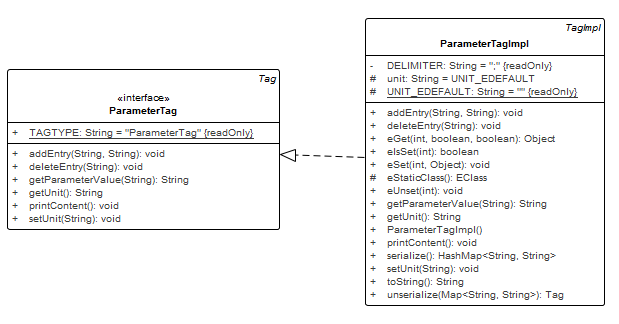
\includegraphics[scale=0.7]{ParameterTag.png}
  		  \caption{Darstellung der Klasse ParameterTagImpl und das Interface ParameterTag}
     \label{uml.ParameterTag}
  \end{center}
\end{figure}


\subsubsection{ParameterTag}
Der Zweck vom Interface \textit{ParameterTag} ist, als Schnittstelle für den Zugriff auf den Inhalt von \textit{ParameterTagImpl} zu dienen. Das Interface erweitert \textit{Tag}. Das \textit{Tag} Interface ist ein in TESTONA allgemein implementiertes Modell, welches auf ein Interface und eine implementierende Klasse basiert (siehe Kapitel \ref{sub.Tags}). In das Interface wurde immer der Tagtyp definiert um \textit{Tags} voneinander unterscheiden zu können.

\begin{lstlisting}
public static final String TAGTYPE = "ParameterTag";
\end{lstlisting}

Das \textit{Tag} wurde um die in Abbildung \ref{uml.ParameterTag} zu sehende Methoden erweitert. Die Konstanten \textit{DELIMETER} (\glqq~| \grqq) und \textit{SEPARATOR} (\glqq~ ; \grqq) wurden benutzt um den Inhalt des Tags beim Speichern und Lesen zu trennen.

\subsubsection{ParameterTagImpl}
Die Klasse \textit{ParameterTagImpl} erweitert die Klasse \textit{TagImpl} und implementiert \textit{ParameterTag}. In dieser Klasse wurden die Vorteile vom Tagmodell deutlicher. Die Klasse \textit{TagImpl} definiert sehr nützliche Methoden und Eigenschaften die in \textit{ParameterTagImpl} weiter angewendet werden.\\


Jedes \textit{Tag} hat als Eigenschaft einen Namen. In dieser Klasse entspricht der Name einem Parameternamen, der aus der Parametertabelle gelesen wurde. Weiterhin ist über \textit{ID} eine eindeutige Identifikationsnummer definiert, um \textit{Tags} des gleichen Typs voneinander unterscheiden zu können. Zwei weitere Attribute wurden  implementiert. Das erste Attribut ist die Einheit (\textit{unit}) des Parameters. Das zweite Attribut ist der Status \textit{merged}. Dieser besagt, ob der \textit{ParameterTag} ein oder mehrere Parameter beinhaltet. \\


Das Attribut \textit{merge} wurde vereinbart, weil ein Baumelement nur ein Objekt pro Tagtyp beinhalten darf. Wenn ein Baumelement zwei oder mehrere Parameter repräsentiert, müssen sich die Werte der Parameter in einen \textit{ParameterTag} befinden. Diese Änderung wurde an den Ansatz (siehe Abbildung \ref{ttn.treeitem_vars}) angepasst.\\


Der Inhalt vom \textit{Tag} ist durch ein \textit{EcoreEMap<String, String>} definiert. Der erste String ist ein Schlüsselwert und der zweite String der Wert. Wenn das \textit{ParameterTag} nur einen Parameter repräsentiert, ist der Schlüssel der Name einer Variante und der Wert ist der Parameterwert des Parameters in dieser Variante. Der Inhalt und Struktur eines \textit{ParameterTags} sieht folgendermaßen aus:\\

\begin{table}[h]
\begin{center}
	\begin{tabular}{|l||ll|}
	 \hline
	 \multicolumn{3}{|c|}{ParameterTag}\\
	 \hline\hline
	 ID			& \multicolumn{2}{|c|}{30}\\
	 \hline
	 Name		& \multicolumn{2}{|c|}{max\_speed}\\
	 \hline
	 Unit		& \multicolumn{2}{|c|}{[km/h]}\\
	 \hline
	 Merged		& \multicolumn{2}{|c|}{false}\\
	 \hline
	 \multirow{5}{*}{Content}	&Key			&Value\\ \cline{2-3}
	 							&Generic		&50\\
	 							&Cabrio		&100\\
	 							&Kombi		&200\\
	 							&Limo		&300\\
	 \hline
	\end{tabular}
	
	\caption{Beispiel eines ParameterTags}
	\label{table:ParameterTagStruktur}
\end{center}
\end{table}


Anhand der Methode \textit{getContent()} wurde der Inhalt eines \textit{Tags} aufgerufen und mit der Methode \textit{addEntry()} wurden Inhalte hinzugefügt. Die Löschung erfolgt mit der Methode \textit{deleteEntry()}. Wie die Methoden genauer angewendet wurden, wird im Listing \ref{lst:CreateParamTag} gezeigt.\\


Wenn ein \textit{ParameterTag} zwei oder mehrere Parameter repräsentiert, sieht die Struktur des \textit{ParameterTags} folgendermaßen aus:

\begin{table}[h]
\begin{center}
	\begin{tabular}{|l||ll|}
	 \hline
	 \multicolumn{3}{|c|}{ParameterTag}\\
	 \hline\hline
	 ID			& \multicolumn{2}{|c|}{31}\\
	 \hline
	 Name		& \multicolumn{2}{|c|}{}\\
	 \hline
	 Unit		& \multicolumn{2}{|c|}{}\\
	 \hline
	 Merged		& \multicolumn{2}{|c|}{true}\\
	 \hline
	 \multirow{3}{*}{Content}	&Key			&Value\\ \cline{2-3}
	 							&speed1|Generic;Cabrio &[km/h]|50;100\\
	 							&speed2|Kombi;Limo     &[km/h]|200;300\\
	 \hline
	\end{tabular}
	
	\caption{Beispiel eines ParameterTags mit zwei Parametern}
	\label{table:PTagMergeStruktur}
\end{center}
\end{table}

Wenn ein Baumelement schon einen \textit{ParameterTag} besitzt, wurden der neue Parameter mit dem aktuellen \textit{ParameterTag} vereinigt. Dafür wurde die Methode \textit{mergeTags (ParameterTag)} definiert. Diese Methode wandelt die Struktur des \textit{ParameterTags} von Tabelle \ref{table:ParameterTagStruktur} zu der Struktur von Tabelle \ref{table:PTagMergeStruktur} um. Die Statusvariable \textit{merge} wurde dann auf \textit{true} gesetzt. Der Inhalt des \textit{ParameterTags} ändert sich auf folgendes Format:

\begin{center}
\begin{tabular}{l l}
Key									&Value\\
\textit{ParameterName}|\textit{Variante1};\textit{Variante2}		&\textit{Einheit}|\textit{Wert1};\textit{Wert2}\\
\end{tabular}
\end{center}


Um ein Parameter aus einem \textit{ParameterTag} mit mehreren Parametern zu löschen, wurde die Methode \textit{removeMergedTag (ParameterName)} programmiert. Die Methode sucht den richtigen Eintrag anhand des Parameternames in \textit{content} und löschst den Eintrag. Falls nur ein Eintrag übrig bleibt, bedeutet es, dass es nur ein Parameter im \textit{ParameterTag} vorhanden ist. Wenn dieser Fall auftritt, wurde die Struktur des \textit{ParameterTags} von Tabelle \ref{table:PTagMergeStruktur} wieder auf die Struktur von Tabelle \ref{table:ParameterTagStruktur} umgewandelt.\\


Sehr relevant sind die Methoden \textit{serialize()} und \textit{unserialize(Map<String, String>)} die für das Schreiben und das Lesen der TESTONA Datei zuständig sind. Zum Schreiben wurde ein \textit{HashMap<String, String>} Objekt zurückgegeben. Das erste \textit{String} beinhaltet den Namen des Parameters gefolgt von den Variantennamen. Der zweite \textit{String} beinhaltet die Einheit des Parameters und die Parameterwerte (in einer geordneten Reihenfolge). Das Format von jedem Eintrag hält sich an das Format von der Tabelle \ref{table:PTagMergeStruktur}. Der XML Eintrag für das obige Beispiel (Tabelle \ref{table:ParameterTagStruktur}) wurde wie folgt aussehen:\\

\begin{lstlisting}[caption={XML Darstellung eines ParameterTags}, captionpos=b]
<Tag id="30" type="ParameterTag">
	<Content key="max_speed|Generic;Cabrio;Kombi;Limo" value="[km/h]|50;100;200;300"/>
<Tag/>
\end{lstlisting}


Beim Laden der TESTONA Datei erkennt das Programm anhand des Attributs \texttt{type} um welchen Typ von \textit{Tag} es sich handelt. Die Methode \textit{unserialize} erhält als Eingansparameter die in \textit{serialize()} erstellte Zeile als ein \textit{Map<String, String>} Objekt. Durch die Trennzeichen (\textit{SEPARATOR} und \textit{DELIMETER}) werden die jeweiligen Werte voneinander unterschieden und den zugehörigen Variablen (name, unit, content) zugeordnet. Beide Vorgänge funktionieren durch die Vererbung automatisiert.

%#######################################################################################
\subsection{ParameterManager}\label{sub:ParameterManager}

\begin{figure}[h]
  \begin{center}
    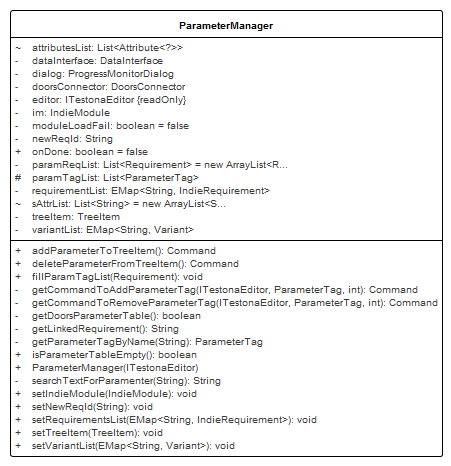
\includegraphics[scale=0.7]{KD_ParameterManager.png}
  		  \caption{Klasse ParameterManager}
     \label{kd.ParameterMananger}
  \end{center}
\end{figure}

Die Klasse \textit{ParameterManager} überprüft und startet die Parameterersetzung. Sie beinhaltet die private innere Klasse \textit{DoorsConnector}. Diese kümmert sich um den Verbindungsaufbau mit DOORS und das Laden von den Parameterwerten aus der Parametertabelle. Die Klasse \textit{DoorsConnector} wird genauer in Kapitel \ref{sub.DoorsConn} erklärt.\\


Mit dem Aufruf der Methode \textit{addParameterToTreeItem()} wird die Parameterersetzung gestartet. Die Methode hat als Rückgabewert ein Kommando, indem ein Parameter hinzugefügt oder gelöscht wird (siehe Kapitel \ref{sub.Command}). Als erstes überprüft die Methode, ob die an das Baumelement verlinkte Anforderung ein Parameter beinhaltet. Falls kein Parameter in der Anforderung gefunden wurde, gibt die Methode den Wert \textit{null} zurück. Wenn ein Parameter gefunden wurde, wird der Name in einer Variablen gespeichert, um diese aus DOORS laden zu können. Wenn noch keine Parameter lokal zu Verfügung stehen (in Form von \textit{ParameterTag} innerhalb einer Liste), wird die Verbindung mit DOORS ge\-startet. Die erforderlichen Angaben zum Verbindungsaufbau befinden sich in der Variable \textit{im} vom Typ \textit{IndieModul} (diese wurde von der Klasse \textit{VariantsManager} gesetzt aus dem \textit{RequirementsConnectionTag}). Das Objekt der Klasse \textit{DoorsConnetor} hat Zugriff auf \textit{im} und kann die gespeicherte Daten abfragen.\\


Während die Verbindung entsteht und die Parametertabelle geladen wird, wird dem Benutzer ein Dialogfenster angezeigt. Die Benutzeroberfläche wird blockiert und zeigt einen Fortschrittsbalken an. Nach einem erfolgreichen Verbindungsaufbau wird die Parametertabelle geladen. Der Pfad zu der Parametertabelle in DOORS ist als Attribut des Hauptmoduls gespeichert. Im Objekt \textit{im} befindet sich der Pfad zum Hauptmodul. Die aktuell implementierte DOORS API in TESTONA kann diese Attribute nicht abfragen. Eine in Moment in Entwicklungszustand neue API wird in der Lage sein, die Attribute abfragen zu können. An dieser Stelle wird als Kompromiss eine Konstante angelegt. In ihr befindet sich der Pfad zur Tabelle.\\

 
Wenn ein Parameter und die zugehörige Werte geladen worden sind, werden sie in \textit{ParameterTag} Objekt gespeichert. Die Methode \texttt{fillParamTagList(Requirement req)} agiert als Parser und wandelt der Übergabeparameter in einen \textit{ParameterTag}. Zu beachten ist, dass innerhalb DOORS jede Zeile in einem Modul als eine Anforderung betrachtet wird. Danach wird die Namensgebung vereinbart und der Übergabeparameter ist vom Typ \textit{Requirement}. Im \textit{Requirement} Objekt befinden sich die Variantennamen und die Parameterwerte. Der folgende Quelltextausschnitt kümmert sich im die Speicherung der Parameterwerte in ein \textit{ParameterTag}.\\


\begin{lstlisting}[caption={Auszug von der Erstellung der ParameterTags}, captionpos=b,label={lst:CreateParamTag}]
ParameterTag tempTag = new ParameterTagImpl();
		
for(int i = 0; i < attributesList.size(); i++){
	
	//An der nullte Stelle steht immer der Parametername
	if(i == 0) {
		tempTag.setName(req.getValue(attributesList.get(0)).getValueAsString());
	} else {
		//Füge ein Eintrag hinzu 
		tempTag.addEntry(sAttrList.get(i),
				req.getValue(attributesList.get(i)).getValueAsString());
	}
}
paramTagList.add(tempTag);
\end{lstlisting}


Die Variable \texttt{attributesList} beinhaltet die in DOORS definierten Varianten.\footnote{Jede Variante in das DOORS Modul wird als ein Attribut definiert und in einer Spalte angezeigt. Wobei nicht jede Spalte des Moduls ein Attribut ist.} Die Liste wird iteriert und die Werte werden im \textit{ParameterTag} gespeichert. Zwei Attribute sind für jedes Parameter in der Liste mindestens definiert. Diese sind der Parametername und ein Standartwert. Möglicherweise ist auch die Einheit des Parameters definiert. Die geladenen Werte werden kontrolliert, ob sie ungleich einen leerer \textit{String} sind.\footnote{Im Ladevorgang einer Anforderung und ihre Attribute in DOORS wird nicht zwischen leeren und befüllte Zellen unterschieden. Der Rückgabewert ist immer ein \textit{String} Wenn die Zelle leer ist, wird ein leerer \textit{String} zurückgegeben.}, bevor sie in ein \textit{ParameterTag} gespeichert werden.\\


Wenn alle vorhandenen Varianten für diesen Parameter iteriert worden sind, wird überprüft, ob der Inhalt (die Variable \textit{content} des \textit{ParameterTags}) der temporären Variable \texttt{tempTag} nicht leer ist. Es kann vorkommen, dass ein Parameter im Modul definiert ist, aber keine weitere Informationen ausgefüllt wurden. Wenn Inhalte vorhanden sind, wird der \textit{ParameterTag} zur einer Liste von \textit{ParameterTags} hinzugefügt.\\

Nachdem die Parameter geladen werden konnten und die Liste befüllt ist, wird die Verbindung mit DOORS geschlossen. Das Dialogfenster wird danach geschlossen und die Benutzeroberfläche wird freigegeben. Während dessen wird in der Liste der richtige \textit{ParameterTag} geladen und die Methode \textit{getCommandToAddParameter()} wird aufgerufen. Diese Methode erzeugt ein Objekt der Klasse \textit{AddParameterTagCommand}. Das zurückgegebene Kommando wird an die Klasse \textit{VariantsManager} weitergeleitet, die wiederum das Kommando an das \textit{ResourceSetListener} weitergibt. Dort wird das Kommando verarbeitet.\\


Für den Fall, dass eine Anforderung aus einem Baumelement gelöscht wird, muss zuerst überprüft werden, ob die Anforderung ein Parameter beinhaltet. Wenn ein Parameter gefunden worden ist, wird das \textit{ParameterTag} aus dem Baumelement geladen. Mithilfe der Klasse \textit{RemoveParameterTagCommand} wird der \textit{ParameterTag} aus dem Baumelement entfernt.

%#######################################################################################
\subsection{Kommandos}\label{sub.Command}
Für das Hinzufügen bzw. Löschen eines Parameters in einem Baumelement wurden zwei Klassen implementiert. Sie erben aus der Klasse \textit{RecordingCommand}. Die Klasse \textit{RecordingCommand} ist eine partielle Implementierung der Klasse \textit{Command}. Diese Klasse nimmt die  Manipulierung der Objekte der Subklasse auf und erzeugt daraus ein Kommando.\footnote{14.02.2015; http://download.eclipse.org/modeling/emf/transaction/javadoc/ 1.2.3/org/eclipse/emf/transaction/RecordingCommand.html} Eine der implementierten Klassen erzeugt ein Kommando für das Hinzufügen eines \textit{ParameterTags} an einem Baumelement,\footnote{AddParameterTagCommand.} während der Zweite für das Löschen zuständig ist.\footnote{RemoveParameterTagCommand.} Der Konstruktor der beiden Klassen hat die gleichen Parameter. Es wird der aktuelle Editor-Objekt übergeben, sowie das Baumelement ID und das \textit{ParameterTag}.\\


Die Methode \textit{doExecute()} wird überschrieben um die Änderung vorzunehmen. Als erstes werden alle Baumelemente geladen und iteriert, bis das Baumelement gefunden wird, das benötigt wird (anhand der ID). Soll ein \textit{ParameterTag} hinzugefügt werden, dann wird die Methode \textit{addTag(ParameterTag pTag)} aufgerufen.\\


Soll ein \textit{ParameterTag} gelöscht werden, dann wird die Methode \textit{removeTag(ParameterTag pTag)} aufgerufen. Danach muss auch der Name des Baumelementes neu gesetzt werden. Wenn ein Baumelement ein Parameter besitzt, je nach aktiver Variante, wird die Darstellung geändert (siehe Kapitel \ref{sec.visualisierung}). Dafür wird der Name des Baumelementes geladen und falls eine Rücksetzung nötig ist, wird diese gemacht. Genaueres dazu wird in Kapitel \ref{sec.LoesungVisualisierung} veranschaulicht.\\

%#######################################################################################
\subsection{Die DOORS Verbindng}\label{sub.DoorsConn}
\subsubsection{DoorsConnector}


Die private innere Klasse \textit{DoorsConnector} baut die Verbindung zwischen TESTONA und DOORS auf. Sie implementiert das Interface \textit{IConnectionListener}, die ein \textit{Listener} für die Verbindungs"=Events umfasst. Für das Laden von Dateien aus DOORS benötigt die Klasse einen zweiten \textit{Listener} (IDataListener) und einen \textit{Adapter} (IReqLoadAdapter). \\

Als erstes wird von der Klasse \textit{ParameterManager} die Methode \textit{connectToDoors()} aufgerufen. Diese baut die Verbindung auf, indem gespeicherte Verbindungsdaten aufgerufen werden. Wie bereits in Kapitel \ref{sub:ParameterManager} erwähnt, beinhaltet eine Anforderung unter anderem die Daten, wo die Anforderung gespeichert ist (welches DOORS Modul und über welches Interface das Modul zu erreichen ist). Für den Verbindungsaufbau werden folgende Objekte benötigt:

\begin{itemize}
\item \textbf{DataInterface: }Über diese Klasse erfolgt die Datenanfrage an DOORS. Die Verbindung wird aufgebaut und auch getrennt. Es werden zuerst die Ordner geladen, danach die einzelnen Projekte und die nötige Module. Es können verschiedene Darstellungen der Module auch geladen werden (diese müssen in DOORS definiert sein). Hier werden auch direkt einzelne Anforderungen angefragt. Relevant für diese Arbeit ist, dass hiermit das Modul Parametertabelle in DOORS geladen wird.

\item \textbf{PreferenceManagment: } Hier werden die in TESTONA gespeicherten Verbindungsdaten behandelt. Es können auch Microsoft Access Verbindungensdaten gespeichert werden, aber wir werden nur DOORS betrachten.

\item \textbf{Connector: }beschreibt eine einzelne Verbindung, hat ein \textit{DataInterface}- und \textit{PreferenceManagmentobjekt}.

\item \textbf{ConnectionManager: }Singleton. Die Klasse handelt aktive und offene Verbindungen. Hier werden die \textit{ConnectionListeners} und das \textit{DataInterface} für den richtigen \textit{Connector} geregelt.

\end{itemize}


Um die Verbindung mit DOORS aufzubauen, muss zunächst die Instanz des \textit{ConnecionManagers} lokal referenziert werden (weil es ein \textit{Singleton} ist, darf kein neues Objekt erzeugt werden). Wenn die Instanz des \textit{ConnectionManagers} geladen ist, kann jetzt der \texttt{connector} aus dem \textit{ConnectionManager} aufgerufen werden.

\begin{lstlisting}[caption={Verbindungsaufbau}, captionpos=b]
try {
	connector = ConnectorManager.getInstance()
				.getConnector(im.getInterId());
	dataInterface = conManager.getNewDataInterface(connector, this);
} catch (ExtensionException e) {
	e.printStackTrace();
}
\end{lstlisting}

 Um dem richtigen \texttt{connector} aufzurufen muss aus dem \textit{IndieModul} (\texttt{im.getInterId()}, siehe Kapitel \ref{sub.VariantsManager}) die Interfacekennung als Übergabeparameter angegeben werden. Dann kann über den \textit{ConnectionManager} ein neues \textit{DataInterface} erzeugt werden. Der \texttt{connector} und das aktuelle Objekt (\textit{DoorsConnector}) werden übergeben.\\
 
Aus den in TESTONA gespeicherten Verbindungspräferenzen werden die Verbindungsparameter für DOORS geladen. An dieser Stelle braucht das \textit{DataInterface} die nötige \textit{Listener} bevor die Verbindung aufgebaut wird. Durch die Methode \textit{addListener(listener)} wird das \textit{RequirementDataListener} und das \textit{IConnectionListener} (von \textit{DoorsConnetor} implementiert) gesetzt. Mit dem Aufruf der Methode \textit{connectInterface(Verbindungsparameter)} wird das \textit{DataInterface} an DOORS verbunden.\\

Der Grund, warum ein \textit{IConnectionListener} implementiert wird, ist, dass der Verbindungsaufbau in einem neuen Thread stattfindet. Das \textit{DoorsConnetor} Objekt wird über den \textit{IConnectionListener} benachrichtigt, ob die Verbindung stattgefunden hat. Die Methode \texttt{interfaceConnected} (aus dem \textit{IConnectionListener}) wird aufgerufen, wenn die Verbindung erfolgreich zustande gekommen ist.

\begin{lstlisting}[caption={Verbindungsaufbau war erfolgreich}, captionpos=b]
@Override
public void interfaceConnected() {
	connected = true;
	reqDataListener.setListener(reqLoadListener);
	dataInterface.loadModule(PARAM_PATH, this, false);
}
\end{lstlisting}

Der gesetzte \textit{RequirementDataListener} benötigt einen \textit{RequirementLoadListener}, dass es eine Rückmeldung gibt, wenn die Zeilen aus einer Tabelle fertig geladen worden sind. Die Tabelle wird anhand der Methode \texttt{loadModule} in ein DOORS Modul (Tabelle) geladen. Welches Modul geladen wird, spezifiziert der Parameter \texttt{PARAM\_PATH}. Es gibt an, wo sich das Modul in der DOORS Datenbank befindet. Der \textit{RequirementDataListener} erhält die Nachricht, dass ein Modul geladen worden ist. Näheres dazu wird im Kapitel \ref{sub.RequirementDataListener} erläutert.\\


Es wird angenommen, dass, wenn der Benutzer einen Parameter ersetzen will, er auch mehrere Parameter ersetzen will. Da die Datenmenge einer Parametertabelle relativ gering ist, wurde hier die Parametertabelle komplett importiert. \\


Ein weiterer Grund besteht, dass nicht für jeden Parameter erneut eine DOORS Verbindung entstehen muss. So wird die Rechen- und Reaktionszeit von TESTONA so gering wie möglich gehalten. Die Parametertabelle wird erst bei der Verknüpfung einer Anforderung mit einem Baumelement importiert und nicht sofort beim Import der Anforderungen. \\


Wenn die Parametertabelle komplett geladen wurde, ermöglicht die Methode \textit{closeConnection} die Verbindung mit DOORS zu beenden und das \textit{DataInterface} zu schließen.





\subsubsection{RequirementDataListener}\label{sub.RequirementDataListener}

Das \textit{RequirementDataListener} ist ein Event-Listener. Dieses Listener wartet auf die Rückmeldung eines Moduls, bis das Modul fertig geladen worden ist. Relevant ist die Methode \texttt{onModuleLoad}, die die Zeilen aus der Tabelle liest und speichert.\\

\begin{lstlisting}[caption={Laden der Parametertabelle nach Zeilen}, captionpos=b]
@Override
public void onModuleLoad(Module module, Object family, boolean reload){

	BasicRequirement baseReq;
	saveAttributesNames(module);
				
	for (String reqId : module.getRequirementIds()) {

		baseReq = dataInterface.getRequirement(module, reqId,
				reqLoadListener);

		if (baseReq.checkStatus(BasicRequirement.STATUS_LOADED)){
			paramReqList.add((Requirement) baseReq);
			fillParamTagList((Requirement) baseReq);
		}
	}
	dataInterface.flush(reqLoadListener);
}
\end{lstlisting}

Zu beachten ist, dass in DOORS jede Zeile in einer Tabelle als eine Anforderung (eng. Requirement) gesehen wird. Daher heißen Variablen und Methoden oft \glqq Requirement\grqq~ oder Abkürzung des Wortes (req). Die Methode \texttt{saveAttributesNames} speichert die im geladenen Modul vorhandenen Attribute. Im diesem Fall anhand mit dem Beispiel Auto sind es:

\begin{itemize}\itemsep1pt
\item Paramenter Name,
\item Default Value,
\item Cabrio Value,
\item Kombi Value,
\item Limo Value.
\end{itemize}

Diese Attribute repräsentieren die Varianten und einen Standardwert und den Name des jeweiligen Parameters. In der Schleife werden alle Zeilen im Modul iteriert und geladen. Wenn die Zeile (\texttt{baseReq}) vollständig geladen wurde, wird diese in der globalen Liste \texttt{paramReqList} als ein \texttt{Requirement} Objekt gespeichert. Die Methode \texttt{fillParamTagList} erzeugt die \textit{ParameterTags} und wird in Kapitel \ref{sub:ParameterManager} erläutert.\\

%Wenn eine Zeile nicht vollständig geladen werden konnte, kümmert sich das \textit{RequirementLoadListener} um das vollständige laden der Zeilen kümmert.
Das \textit{RequirementLoadListener} wird in dieser Klasse instanziiert und von der \textit{DoorsConnetor} Klasse gesetzt. Weiter dazu im nächsten Kapitel.


\subsubsection{RequirementLoadListener}\label{sub.RequirementLoadListener}
Der \textit{RequirementLoadListener} reagiert, wenn eine Zeile nicht völlstandigt geladen worden ist, und wartet bis diese geladen wird. Die Methode \texttt{onLoad} bekommt als Eingabeparameter eine Liste der nicht geladenen Zeilen.

\begin{lstlisting}[caption={Nachladen der Parametertabelle nach Zeilen}, captionpos=b]
public void onLoad(List<BasicRequirement> requirements) {

	for (BasicRequirement baseReq : requirements) {
		paramReqList.add((Requirement) baseReq);
		fillParamTagList((Requirement) baseReq);
		
	}
}
\end{lstlisting}

Diese Liste wird iteriert und wie in \textit{RequirementDataListener} in der globalen Liste \texttt{paramReqList} als ein \texttt{Requirement} Objekt gespeichert.\\

Weiterhin meldet diese Klasse, wenn alle Zeilen aus dem DOORS Modul geladen wurden. Das wartende Dialogfenster aus \ref{sub:ParameterManager} wird benachrichtigt, dass es geschlossen werden kann. Die Benutzeroberfläche von TESTONA ist somit wieder für den Benutzer erreichbar.



%#######################################################################################
%#######################################################################################
\newpage
\section{Darstellung der Parameterwerte}\label{sec.LoesungVisualisierung}
\paragraph{}

Nachdem Parameter in den Baumelementen vorhanden sind, sollten die Werte angezeigt werden. Wenn ein Pfeil oder die Kombo-Box (siehe Kapitel \ref{sec.visualisierung}) für eine Änderung der Variantenansicht betätigt werden, muss jedes Baumelement überprüft werden. Gibt es einen gültigen Wert für die aktive Variante, muss dieser angezeigt werden.\\

 
\begin{table}[h]
\begin{center}
	\begin{tabular}{|l||ll|}
	 \hline
	 \multicolumn{3}{|c|}{ParameterTag}\\
	 \hline\hline
	 Name		& \multicolumn{2}{|c|}{max\_speed}\\
	 \hline
	 Unit		& \multicolumn{2}{|c|}{[km/h]}\\
	 \hline
	 \multirow{5}{*}{Content}	&Key			&Value\\ \cline{2-3}
	 							&Generic		&50\\
	 							&Cabrio		&100\\
	 							&Kombi		&200\\
	 							&Limo		&300\\
	 \hline
	\end{tabular}
	\caption{Parameter \textit{max\_speed}}
	\label{table:ParameterTagStruktur2}
\end{center}
\end{table}


\begin{figure}[h!]
\centering
\begin{minipage}{.5\textwidth}
  \centering
  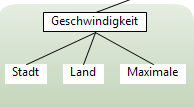
\includegraphics[width=.4\linewidth]{52Generic.png}
  \caption{Der generische Baum}
  \label{ttn.52Generic}
\end{minipage}%
\begin{minipage}{.5\textwidth}
  \centering
  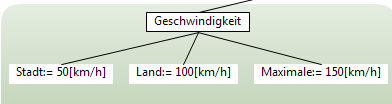
\includegraphics[width=.8\linewidth]{52Cabrio.png}
  \caption{Aktive Variante Cabrio}
  \label{ttn.52Cabrio}
\end{minipage}
\end{figure}


\begin{figure}[h!]
\centering
\begin{minipage}{.5\textwidth}
  \centering
  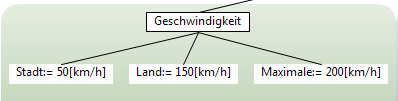
\includegraphics[width=.8\linewidth]{52Limo.png}
  \caption{Aktive Variante Limo}
  \label{ttn.52Limo}
\end{minipage}%
\begin{minipage}{.5\textwidth}
  \centering
  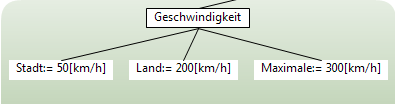
\includegraphics[width=.8\linewidth]{52Kombi.png}
  \caption{Aktive Variante Kombi}
  \label{ttn.52Kombi}
\end{minipage}
\end{figure}


Wenn die Einheit des Parameters definiert ist, wird diese auch angezeigt. Zwischen Baumelementname und dem Wert befinden sich die Zeichen \glqq :=\grqq~ als Trennzeichen. Diese Maßnahme wurde eingeführt, da Baumelemente unter einem Knoten nicht den gleichen Namen besitzen dürfen. So kann das Programm und der Benutzer jedes Baumelemente eindeutig identifizieren.\\


Nachdem einer der Schaltflächen zum Ändern der Variantenansicht betätigt wird, wird die Methode \textit{activateVariant()} in der Klasse \textit{VariantsManager} aufgerufen. Innerhalb der Methode werden alle Baumelemente, falls es nötig ist, neu benannt. \\


Die Umbenennung der Baumelemente erfolgt, wie beim Hinzufügen eines \textit{ParameterTags}, über ein Kommando. Im diesem Fall wird kein Objekt des Typs \textit{Command} zurückgegeben, sondern die Methode \textit{executeEMFCommand} bekommt als Parameter das Kommando. Die Methode hängt das Kommando an den Stack und verhindert, dass das Kommando vom \textit{Garbage Collector} gelöscht wird.\\


Das Kommando ist eine Klasse in der die \textit{ParameterTags} ausgewertet werden. Wenn das Baumelement ein \textit{ParameterTag} hat, wird überprüft ob für die aktive Variante ein Parameterwert definiert ist. Wenn ein Parameterwert gefunden wurde, wird das Baumelement immer mit dem folgenden Format neu benannt:

\begin{center}
\textit{name} := \textit{wert}[\textit{einheit}]
\end{center}

Wobei nur \textit{einheit} ein optionaler Wert ist. Falls kein Parameterwert für die Variante definiert wurden ist wird der Standartname angezeigt (\textit{name}).\\

Alle Baumelemente müssen aus zwei Gründen geprüft werden. Der erste Grund ist, dass nicht für alle Varianten Parameterwerte zur Verfügung stehen können. Der zweite Grund ist, dass eine Anforderung aus einem Baumelement gelöscht werden kann, nachdem die Werte schon angezeigt worden sind. In beiden Fällen muss der Name des Baumelements auf den Standartname gesetzt werden.\\


Nachdem alle Baumelemente überprüft worden sind, muss die Anzeige (Editor) von TESTONA aktualisiert werden. Durch das Ändern der Namen, ändert sich auch die Breite der Baumelemente und diese müssen neu organisiert werden. Danach wird der Befehl gegeben die Anzeige neu zu zeichnen. Das Ergebnis wird in den Abbildungen \ref{ttn.52Generic} bis \ref{ttn.52Kombi} dargestellt.



%#######################################################################################
%#######################################################################################
%\newpage
%\section{Testfallgenerierung und Optimierung}
%\paragraph{}
%Erläuterung der Lösungen zu 4.3